\newpage
\section{Inference on Lee-Carter Model with Inlabru - Preliminary Test with Synthetic Data}
We investigate whether a linearization of the non-linear predictors $\eta_{x,t}$ in the Lee-Carter models will enable usage of \inla to perform Bayesian inference on these models. We follow the linearization scheme proposed by \textcite{BachlLindgren2019}, and use the \inlabru library in \texttt{R} to perform the linearization and iterative runs of the \inla-method. In the first part of our investigation, we apply the methodology to synthetic data. The advantage of using synthetic data to test this method is that we know the exact model from which the data are sampled, and we are then able to determine whether the model approximated by \inlabru is close to the real (synthetic) model. 

\subsection{Implementation of \inlabru}
\label{sec:implementationInlabru}
The \inlabru library is a wrapper around the more commonly used \rinla library. The implementation of Bayesian inference in the \inlabru library is similar to that of the \rinla library, with some syntactic differences. For an extensive introduction to the \rinla library we refer to the book by \textcite{Rubio2020}. Further references to the \inlabru library can be found at \textcite{Inlabru}. Here, we will briefly cover the main parts of code needed to use the \inlabru library to perform Bayesian inference. All code used and discussed in this paper can be found at \url{https://github.com/Helenerb/Project-thesis}. 
\newline
\noindent The following parts are needed to implement Lee-Carter types of models in \texttt{R} and run \inlabru with it:
\begin{itemize}
    \item a data frame containing the observations and the corresponding covariate values
    \item a definition of the components that may be included in the formula for the likelihood. For the model in \ref{eq:LC-rewritten}, these will be $\alpha_x$, $\beta_x$, $\kappa_t$, $\phi$, $\epsilon_{xt}$ and the intercept $\mu$.
    \item the definition of the likelihood formula, using the components described above.
\end{itemize}
When all the above-mentioned parts are defined, \inlabru can be run using the command 
\begin{verbatim}
    res = bru(components = comp,
          likelihood, 
          options = list(/*Your desired options*/)).
\end{verbatim}
A data frame with the results from the approximation will be stored in the \texttt{res} variable. 
\newline
\subsection{First Test of Inference with \inlabru on LC-model}
\label{sec:synthFirstInferenceLC}
\noindent To produce the synthetic data, we choose functions for $\alpha_x$, $\beta_x$ and $\kappa_t$ and a $\phi$ that we believe to be somewhat realistic: $\alpha_x$ is modeled both as a constant (i.e. included in the intercept $\mu$) and as different functions and realizations of random walks, $\kappa_t$ are modeled as different functions and realizations of random walks and $\beta_x$ is modeled as 
\begin{equation*}
    \beta_x \sim \Normal(0,1/\tau)
\end{equation*} 
for some precisions $\tau$. We sample the random terms $\epsilon_{x,t}$ from an iid normal distribution with zero mean and precision $\tau_\epsilon$. $\alpha_x$, $\beta_x$ and $\kappa_t$ are then scaled to their respective constraints, given in \ref{eq:LCconstraintsFinal}. As we expect \inlabru to handle any sufficiently smooth and close-to-realistic effects to accept it as a suitable inference tool for the LC and LCC model, we do not attach a lot of importance to the choices for the synthetic models for the random effects. 
The \inlabru method was run for multiple configurations of the true effects. Figure \ref{fig:firstRun} displays the results from the run when the random effects were modelled as
\begin{equation}
    \begin{aligned}
    \alpha_x &= \cos(\frac{x-3}{6}\pi)\\
    \beta_x &= \Normal(0,0.1^2)\\
    \phi &= -0.5\\
    \kappa_t &= 0.3\cos(\frac{t\cdot \pi}{5})\\
    \tau_{\epsilon} &= 1/0.01^2.
    \end{aligned}
    \label{eq:conf21}
\end{equation}
for $x\in [1,10]$ and $t \in [1,10]$. The code used to produce these results can be found at the \texttt{GitHub} repository under \texttt{synthetic-data/L-C-alpha-x.R}. 
\begin{figure}[h!]
    \centering
    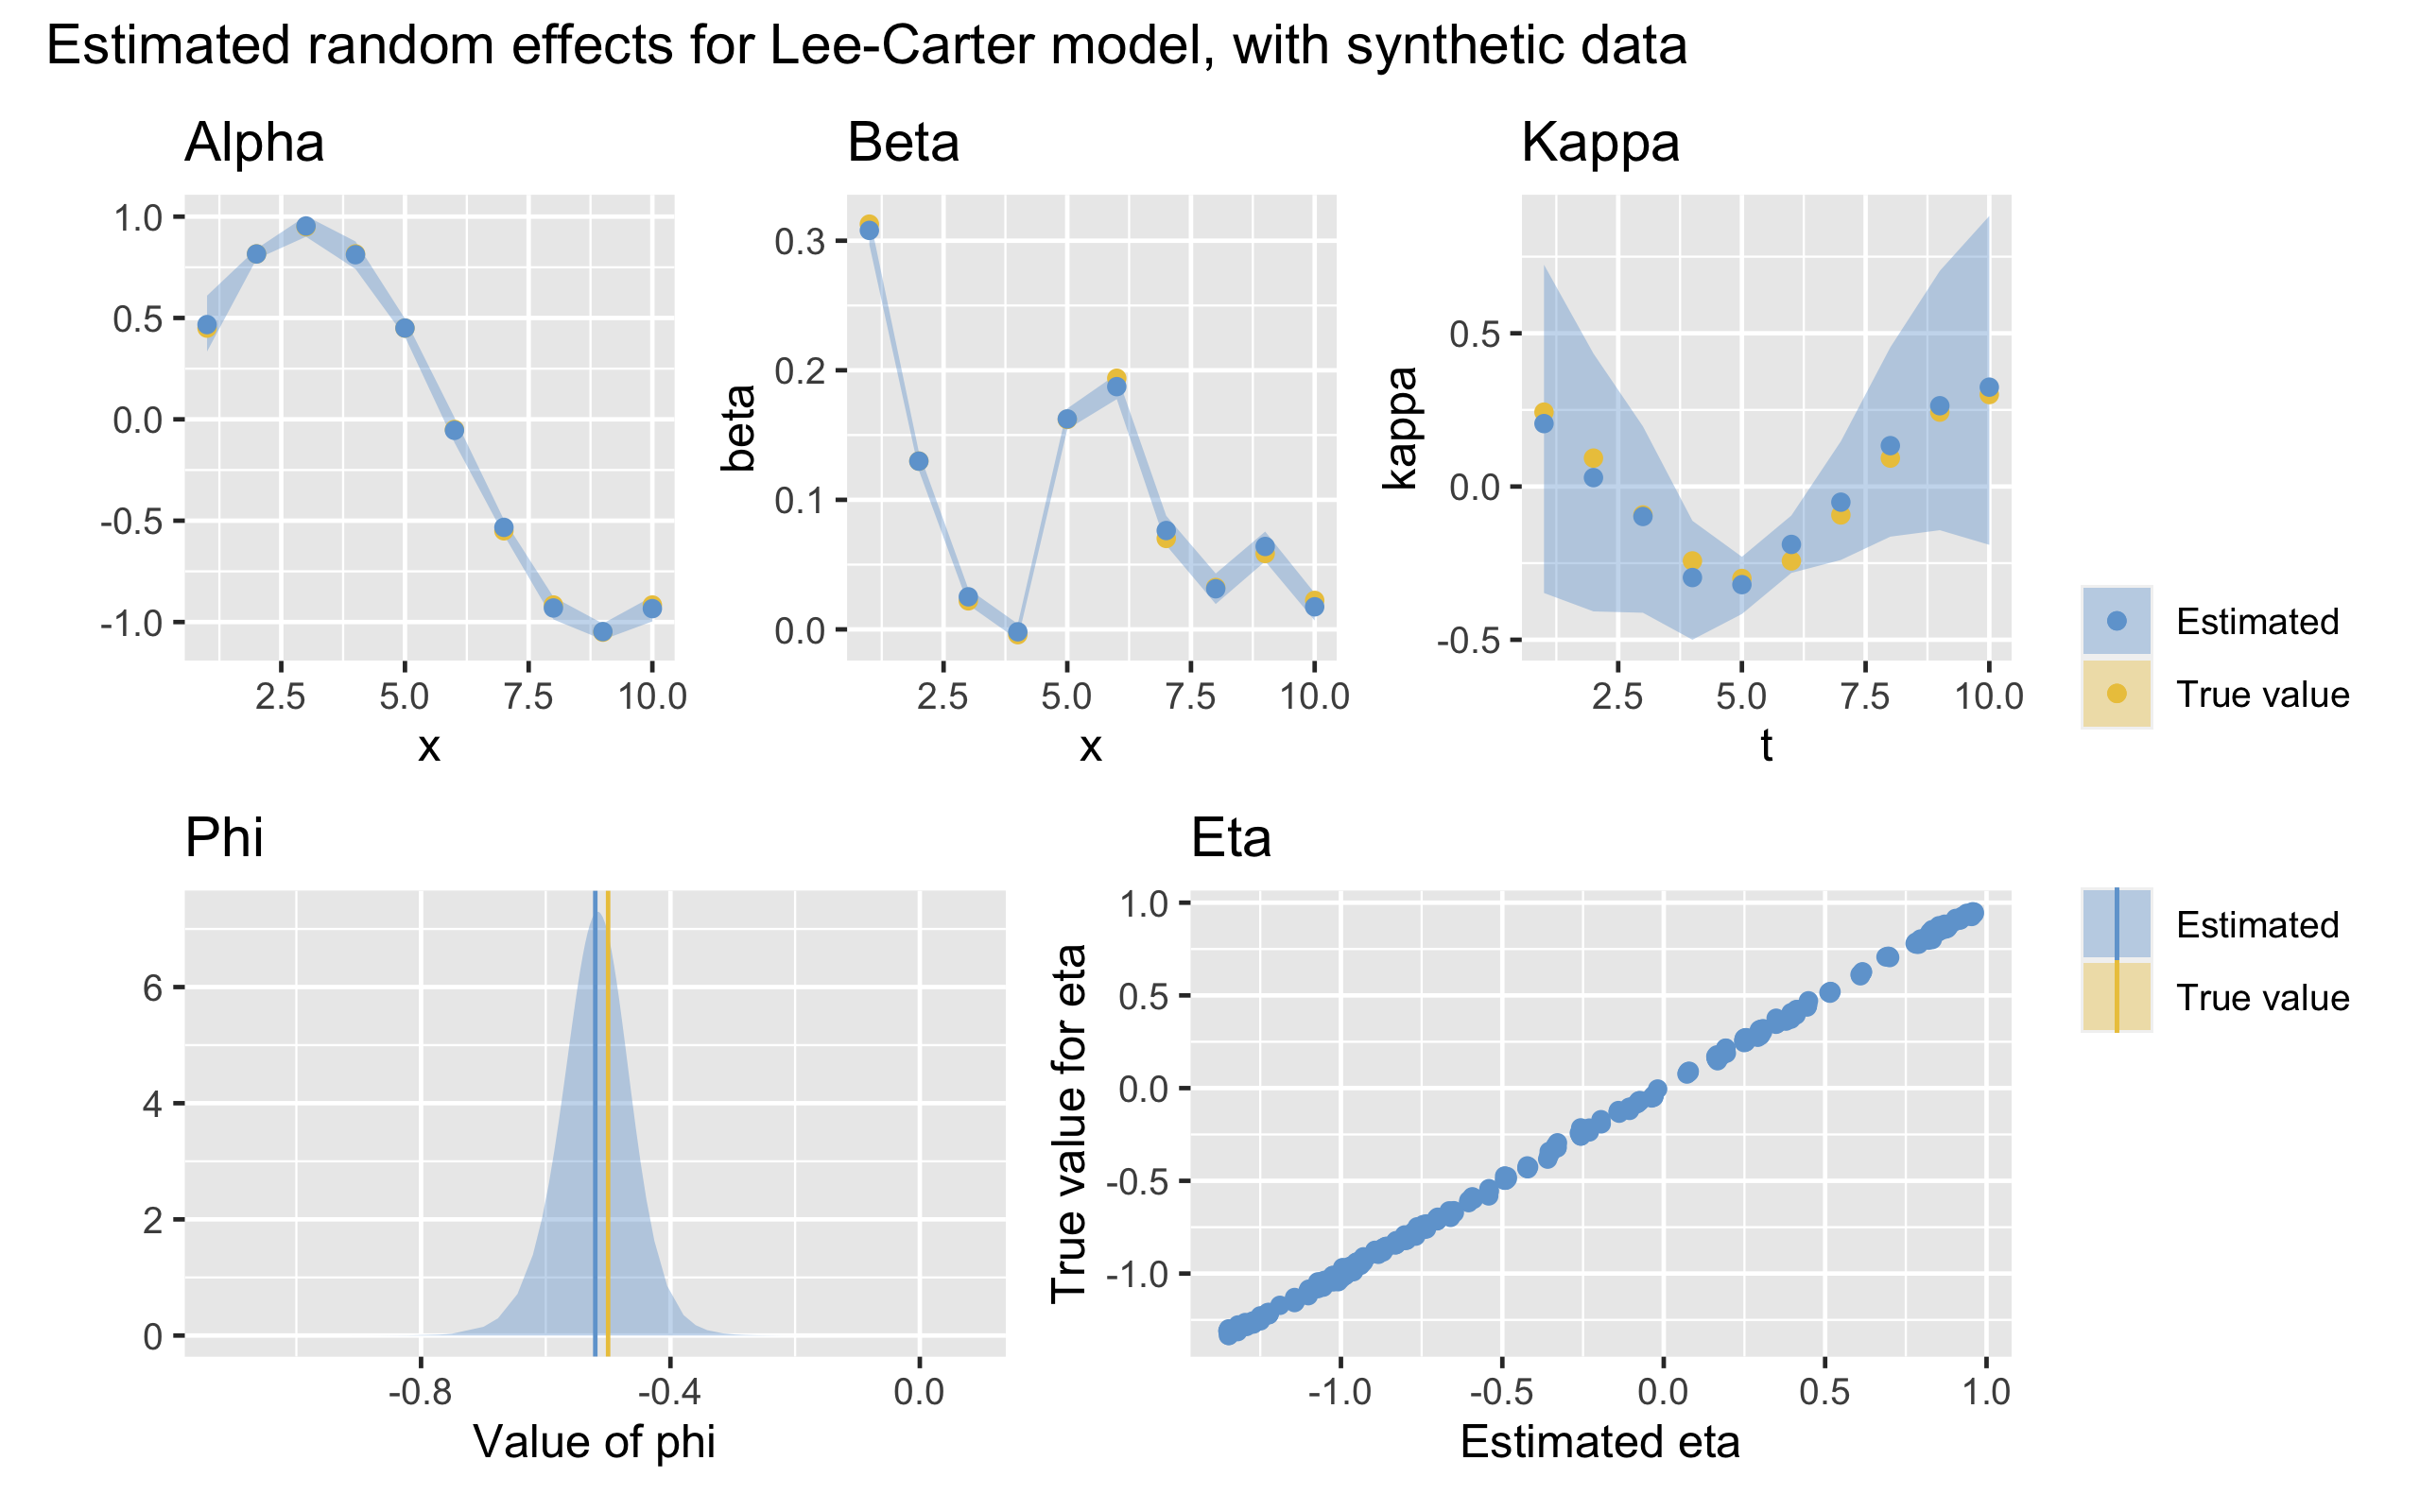
\includegraphics[width=0.85\linewidth]{synthetic-data/Figures/effects-LC-synthetic.png}
    \caption{The results from running \inlabru when the random effects are simulated from the model given in Expression \ref{eq:conf21}. \textit{Top:} The mean and the 95\% confidence bounds of the approximated posterior marginal distributions of $\alpha_x$ (Alpha), $\beta_x$ (Beta) and $\kappa_t$ (Kappa), together with their respective true random effects. \textit{Bottom, left:} The approximated marginal posterior distribution of $\phi$ with the mean value as a solid line, together with the true value of $\phi$. \textit{Bottom, right:} The mean of the approximated posterior marginal distribution for $\eta_{x,t}$ plotted against the true value for $\eta_{x,t}$. }
    \label{fig:firstRun}
\end{figure}
From Figure \ref{fig:firstRun} it is clear that \inlabru is able to identify all random effects significantly, as well as displaying a good estimation for the predictor $\eta_{x,t}$ (A straight line with a slope of one in the plot of estimated and true values of $\eta_{x,t}$ correspond to equal values). Looking at the results from testing \inlabru with other models for the random effects, we observe that \inlabru is able to produce a good result for the predictor $\eta_{x,t}$ in all cases and good results for the random effects in most cases. In Section \ref{sec:IdentifiabilityKappa} we discuss why the combination of random effects that yield bad results from \inlabru are not considered realistic, and then not a hinder for using \inlabru to fit LC-models. These results provide the basis for for our paper, as it shows that \inlabru makes it possible to bypass the obstacle that \inla alone is not able to handle Lee-Carter type handle models with non-linear predictors.

\subsection{Choice of Implementation of $\beta_x$}
\textcolor{myDarkGreen}{This is actually a quite important part. Be quite technical, include the two different code snippets. }
In the implementation of the LC-model (\ref{eq:LC-rewritten}) in \texttt{R}, the multiplicative term of the predictor $\etax$ is entered as
\begin{equation}
    \beta_x\cdot\phi \cdot t + \beta_x\kappa_t,
\end{equation}
so that the $\beta_x$ effect exists in two terms. \inla (and then also \inlabru) offers two ways to handle this. The first option is to use the same component for $\beta_x$ in both terms, which is implemented (for the simplest LC-model where $\alpha_x$ is included in the intercept) in the \texttt{components} object and the \texttt{formula} object as:
\begin{verbatim}
comp.single = ~ Intercept + 
    phi(t, model = "linear") + 
    beta(x, model = "iid", extraconstr = list(A = A.mat, e = e.vec)) + 
    kappa(t1, model = "rw1", values = 1:nt, constr = TRUE, hyper = pc.prior) + 
    epsilon(xt, model = "iid")
form.single = y ~ Intercept + beta*phi + beta*kappa + epsilon
\end{verbatim}
In Section \ref{sec:synthFirstInferenceLC} this implementation was used. The second option is to define two different components for $\beta_x$, and to use the \texttt{copy}-feature in \inla to make one component a copy of the other, plus some noise \cite{MARTINS201368}. This is implemented as
\begin{verbatim}
comp.copy = ~ Intercept + 
    phi(t, model = "linear") + 
    beta1(x, model = "iid", extraconstr = list(A = A.mat, e = e.vec)) + 
    kappa(t1, model = "rw1", values = 1:nt, constr = TRUE, hyper = pc.prior) + 
    beta2(x1, model = "iid", copy="beta1") +
    epsilon(xt, model = "iid")
form.copy = y ~ Intercept + beta1*phi + beta2*kappa + epsilon
\end{verbatim}
We investigate whether both approaches can be used to fit our model, and if so, which one performs the best. The code used to produce these results can be found at the \texttt{GitHub} repository under \texttt{synthetic-data/L-C-copy-beta.R}. 

\begin{figure}[h!]
    \centering
    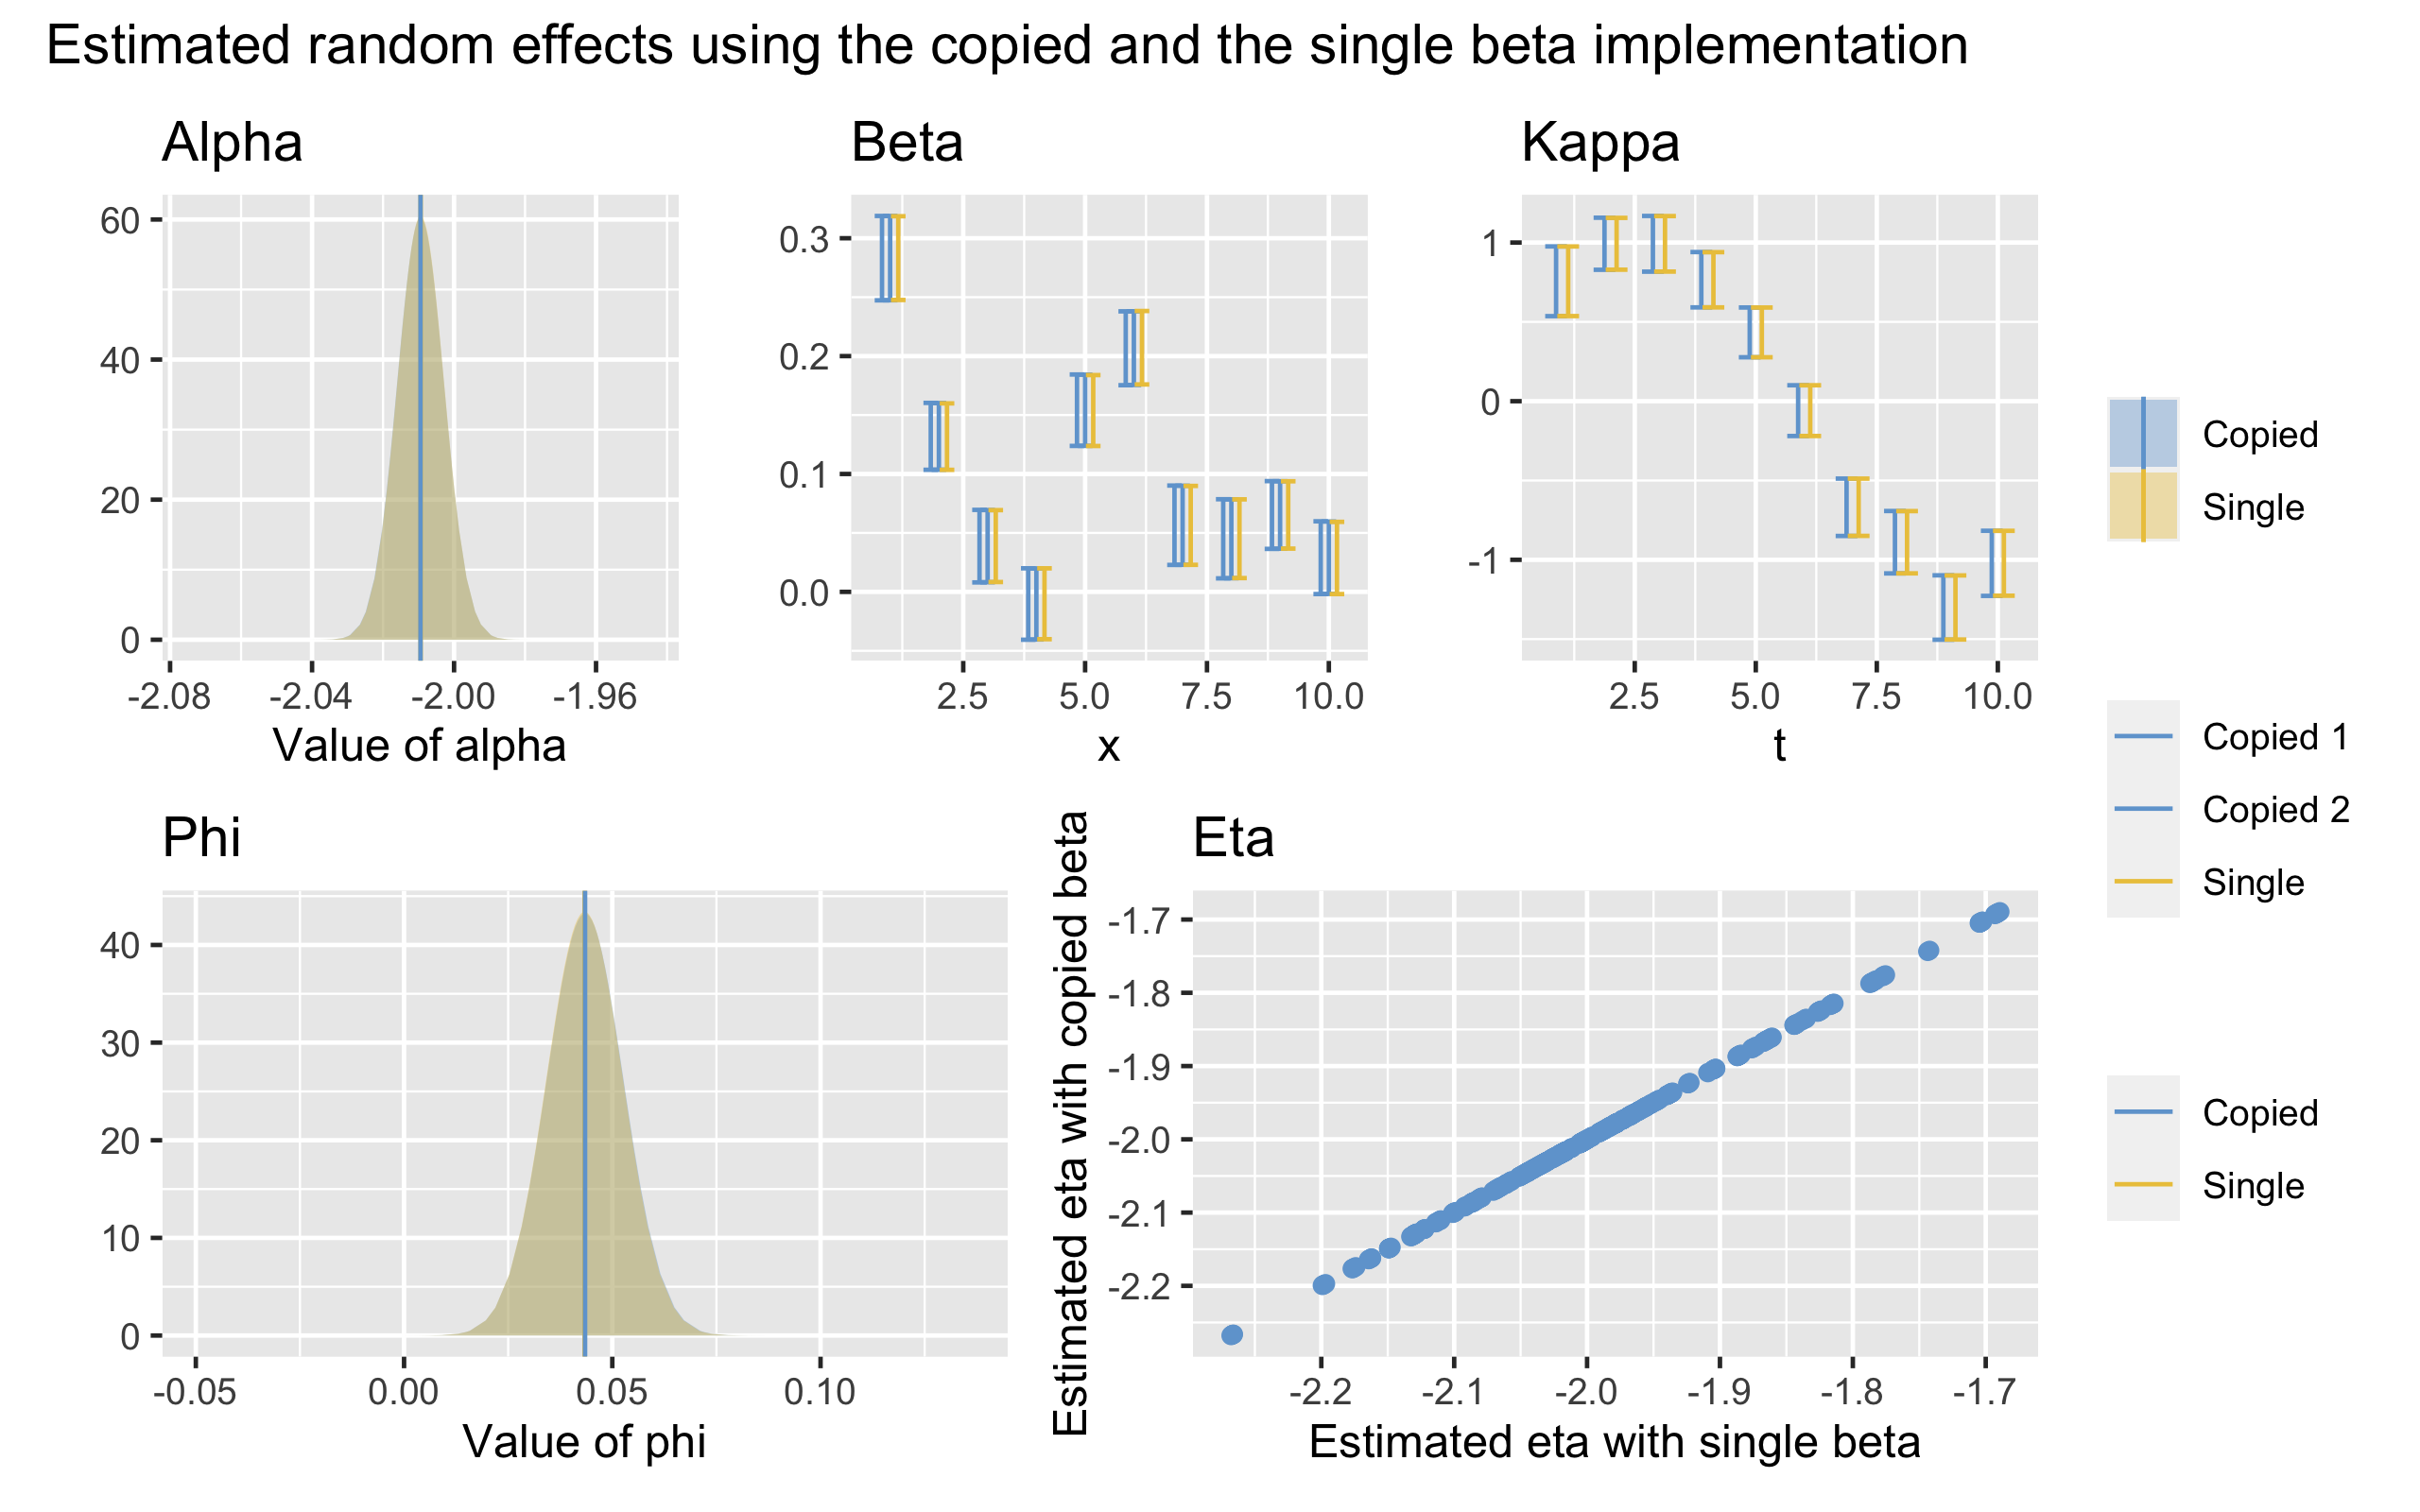
\includegraphics[width=0.85\linewidth]{synthetic-data/Figures/copy-beta.png}
    \caption{\textit{Top:} The posterior marginal distributions for $\alpha_x$, and the 95\% confidence bounds for the marginal posteriors of $\beta_x$ and $\kappa_t$, with and without the \texttt{copy} feature. \textit{Bottom, left:} The approximated marginal posterior distribution of $\phi$ with the mean value as a solid line, with and without the \texttt{copy} feature. \textit{Bottom, right:} The mean of the approximated posterior marginal distribution for $\eta_{x,t}$ from the implementation with the \texttt{copy} feature plotted against the true value for $\eta_{x,t}$ from the implementation without the \texttt{copy} feature. }
    \label{fig:copyBetaComparison}
\end{figure}

\begin{figure}[h!]
    \centering
    \begin{subfigure}[b]{0.45\textwidth}
        \centering
        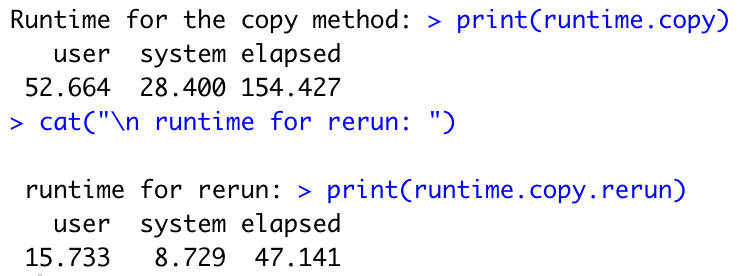
\includegraphics[trim=0 5 0 0,clip,width=\textwidth]{synthetic-data/Figures/runtime-copy.png}
    \end{subfigure}
    \begin{subfigure}[b]{0.45\textwidth}
        \centering
        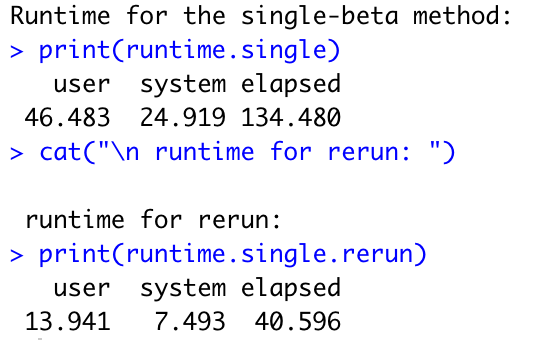
\includegraphics[trim=0 0 15 0,clip, width=\textwidth]{synthetic-data/Figures/runtime-single.png}
    \end{subfigure}
    \caption{The run time of running \inlabru inference using the $\texttt{copy}$-feature (right) and without using the $\texttt{copy}$-feature (left).}
    \label{fig:copyBetaRuntimes}
\end{figure}

A comparison between the results from the two runs with the different implementations are displayed in Figure \ref{fig:copyBetaComparison} and the corresponding run times are shown in Figure \ref{fig:copyBetaRuntimes}. We do not observe any difference in the accuracy of the results from the two implementations, they seem to produce exactly the same results. From Figure \ref{fig:copyBetaRuntimes} we observe that the implementation using the $\texttt{copy}$-feature seemed to take slightly more time to run. Even through this difference in run time is not necessarily significant, we still do not want to unnecessarily complicate our implementations, and we do not use the \texttt{copy}-feature in the remaining simulations.

\subsection{Identifiability Issues with $\kappa_t$ and $\phi\cdot t$}
\label{sec:IdentifiabilityKappa}
For some combinations of underlying models for $\kappa_t$ and $\phi$ we observe that \inlabru is not able to correctly identify these effects, while the prediction of $\etav$ is still correct, as mentioned in Section \ref{sec:synthFirstInferenceLC}. This indicates that there are some identifiability issues between $\kappa_t$ and $\phi \cdot t$ that become apparent for some combinations of these effects. We test several different combinations of $\kappa_t$ and $\phi$ to try to isolate the types of combinations that \inlabru is not able to correctly identify.
\begin{figure}[h!]
    \centering
    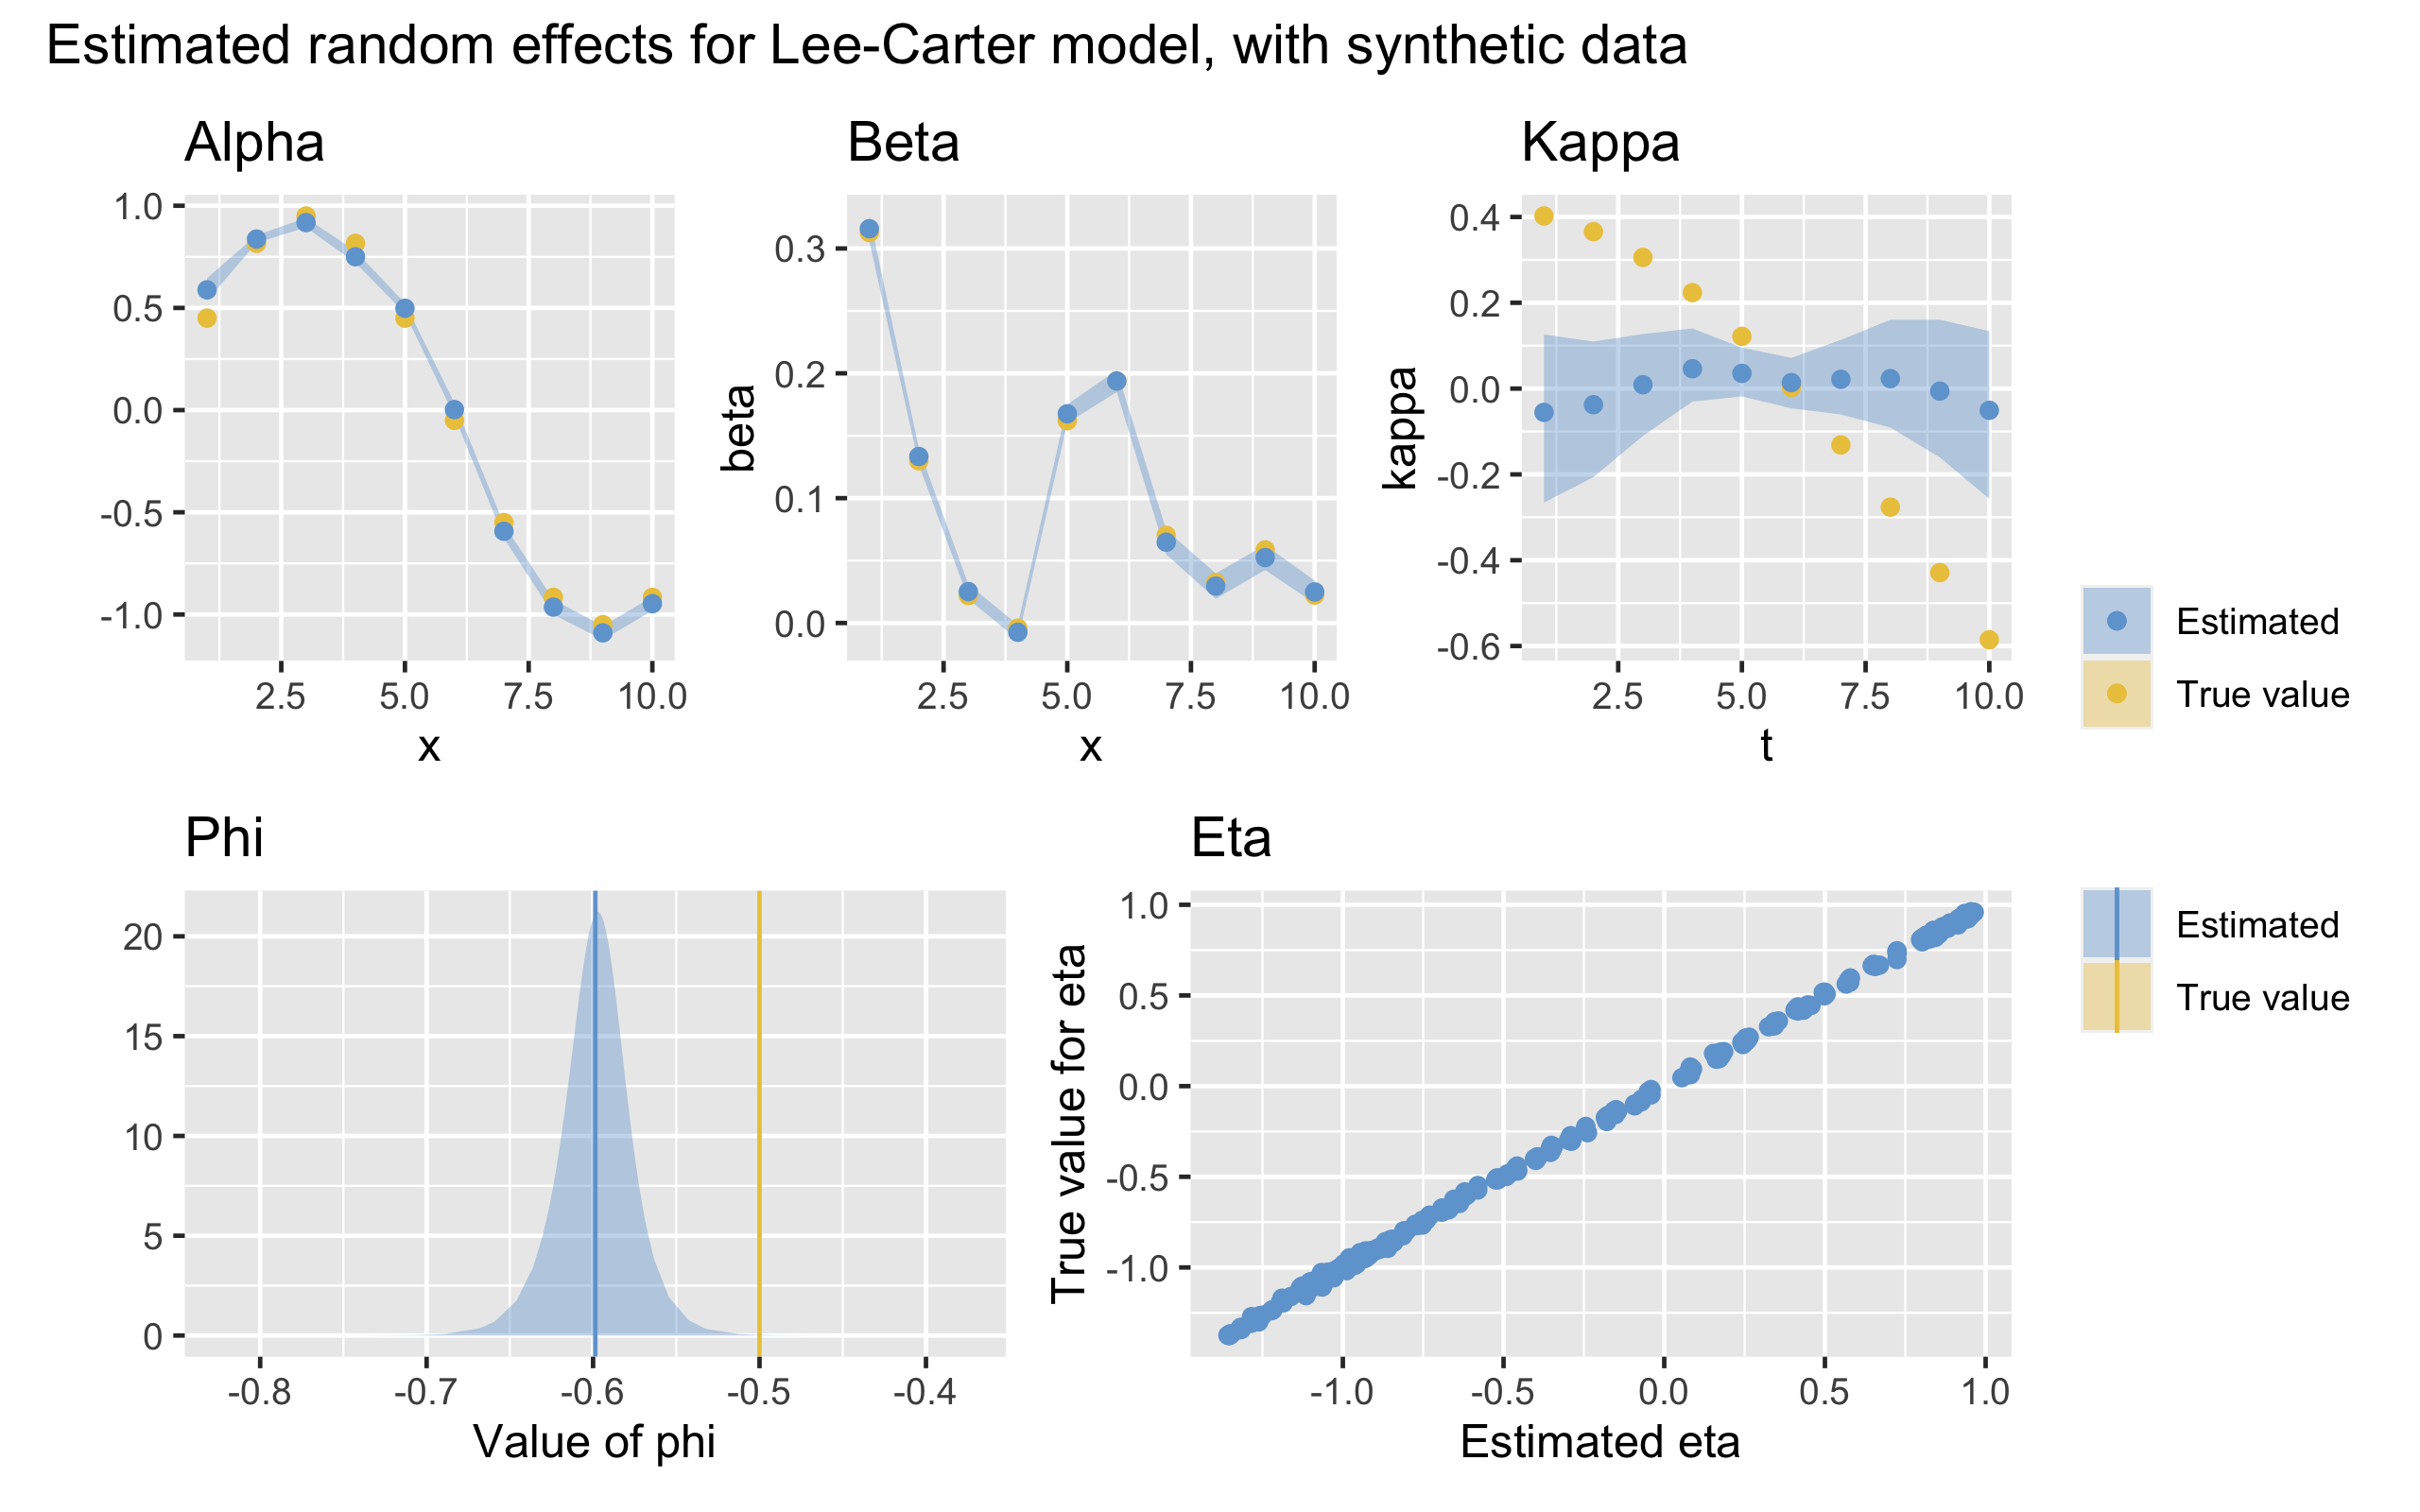
\includegraphics[width=0.85\linewidth]{synthetic-data/Figures/effects-LC-synthetic-identifiability.png}
    \caption{An example of the results after running \inlabru with a configuration that yields identifiability issues with $\kappat$ and $\phi \cdot t$. The plot layout is similar to that of Figure \ref{fig:firstRun}.}
    \label{fig:unidentifiabilityKappa}
\end{figure}
Figure \ref{fig:unidentifiabilityKappa} displays the results from running \inlabru on the following configuration of random effects:
\begin{equation}
    \begin{aligned}
    \alpha_x &= \cos(\frac{x-3}{6}\pi)\\
    \beta_x &= \Normal(0,0.1^2)\\
    \phi &= -0.5\\
    \kappa_t &= \cos(\frac{t\cdot \pi}{20})\\
    \tau_{\epsilon} &= 1/0.01^2.
    \end{aligned}
\end{equation}
for $x\in[1,10]$ and $t\in[1,10]$. The code used to produce these results can be found at the \texttt{GitHub} repository under \texttt{synthetic-data/L-C-alpha-x.R}. From Figure \ref{fig:unidentifiabilityKappa} we clearly see errors in the approximations of $\kappav$ and $\phi\cdot t$ while the approximations of $\etav$ (and $\betav$ and $\alphav$) are close to the true values. We observe, from these and other similar results, that \inlabru produces incorrect models for $\kappa_t$ and $\phi$ when the underlying model for $\kappa_t$ show too clear drift tendencies. This indicates that \inlabru places all drift along the period axis in the linear term $\phi$. We can accept this "misplacement", since we have explicitly defined our model as the sum of a random walk without drift and and some linear effect. Even though the realization of a drift-less random walk could easily display drift-like tendencies, we accept the apparent assumption of \inlabru that all drift along the $t$ axis originates from the linear effect $\phi \cdot t$, since we still get good results for the predictor $\eta_{x,t}$ and the remaining random effects.
\newline
\subsection{Inference with \inlabru on the LCC-model. }
The next step in our preliminary analysis is to test the performance of \inlabru on the LCC-model, as defined in \ref{eq:LCC-rewritten}. The cohort effect is included in the \texttt{R} script in the same manner as the other effects. As in the previous phase, \inlabru was tested on several different realizations of the true model. All code used in this phase can be found at \url{https://github.com/Helenerb/Project-thesis/synthetic-data} in the scripts \texttt{L-C-cohort-rw.R} and \texttt{L-C-cohort-v2.R}.
\begin{figure}[h!]
    \centering
    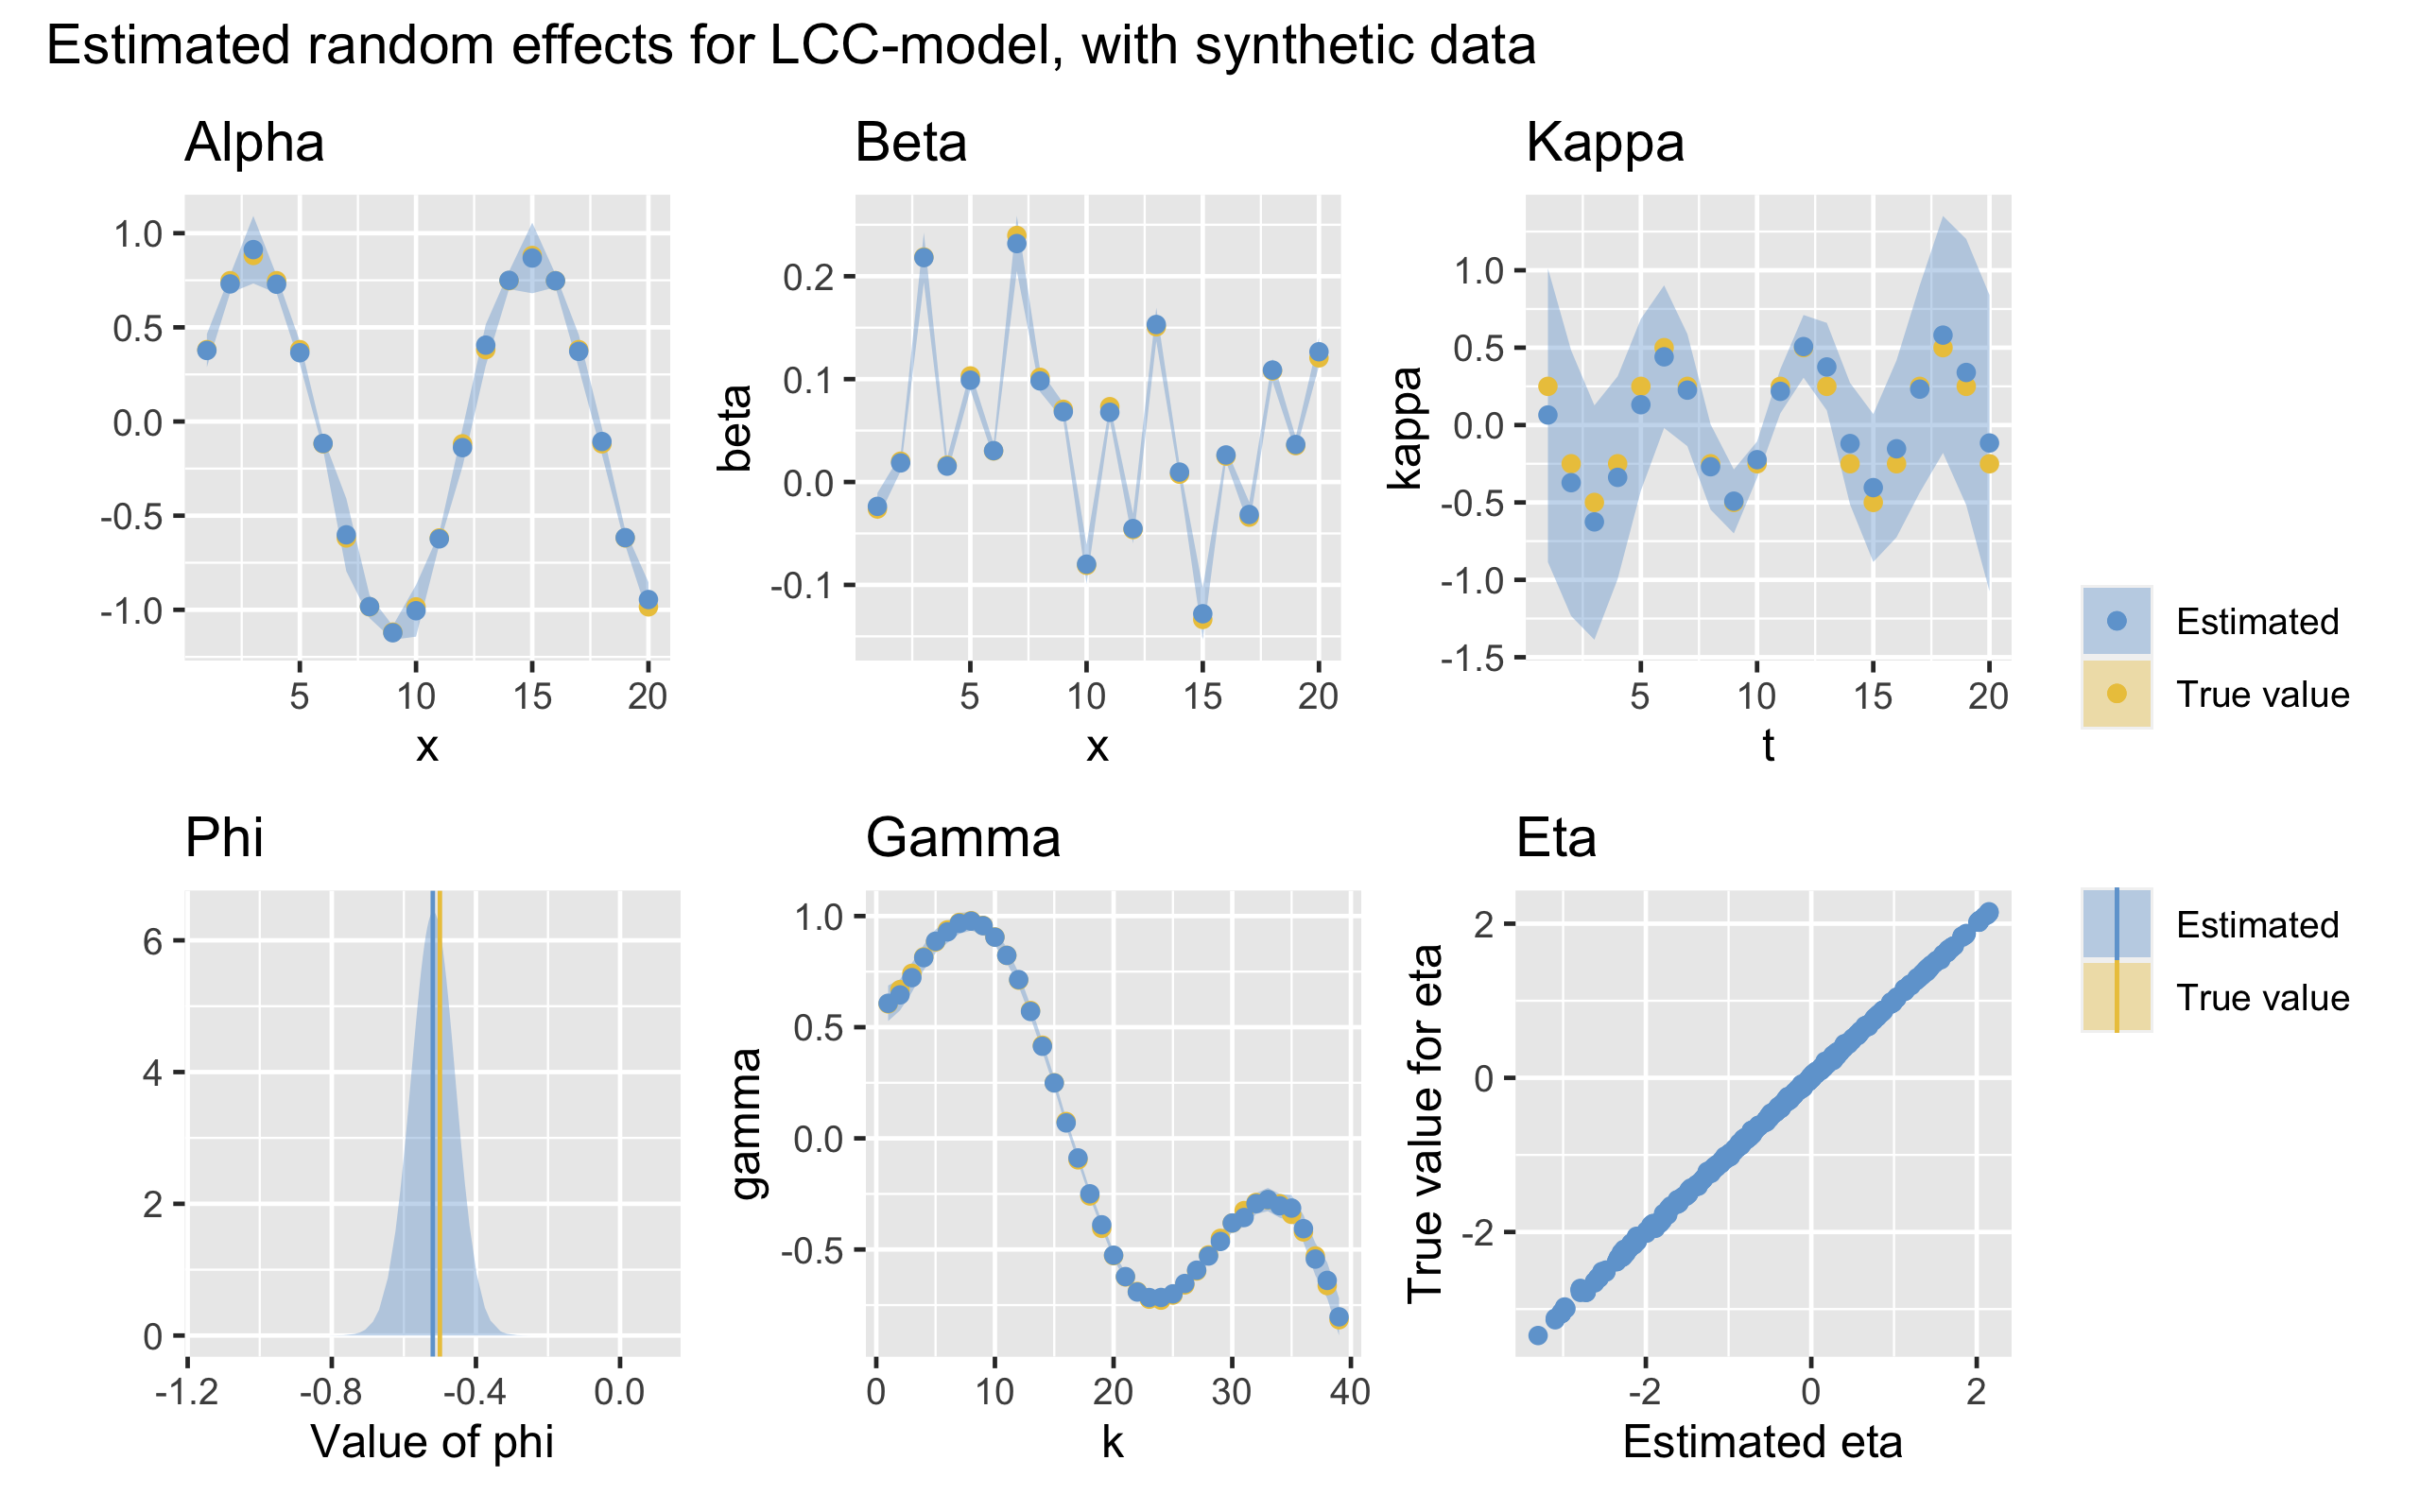
\includegraphics[width=0.85\linewidth]{synthetic-data/Figures/effects-LCC-synthetic-3-1.png}
    \caption{Results from running \inlabru with the configuration of random effects given in Expression \ref{eq:conf31}. The plot layout is similar to that of Figure \ref{fig:firstRun}.}
    \label{fig:conf31}
\end{figure}
Figure \ref{fig:conf31} displays the results from running \inlabru with the following configuration of random effects:
\begin{equation}
    \begin{aligned}
        &\alpha_x = \cos(\frac{x-3}{6}\pi)\\
        &\beta_x = \Normal(0,0.05^2)\\
        &\phi = -0.5\\
        &\kappa_t = \frac{1}{2}\cos(\frac{t\cdot \pi}{3})\\
        &\gammax = -\frac{1}{2}\left( 0.1k + \cos(\frac{k-2}{4})\right)\\
        &\tau_{\epsilon} = 1/0.01^2.
    \end{aligned}
    \label{eq:conf31}
\end{equation}
for $x\in[1,20]$, $t \in [1,20]$ and $k \in [1,39]$. 

\begin{figure}[h!]
    \centering
    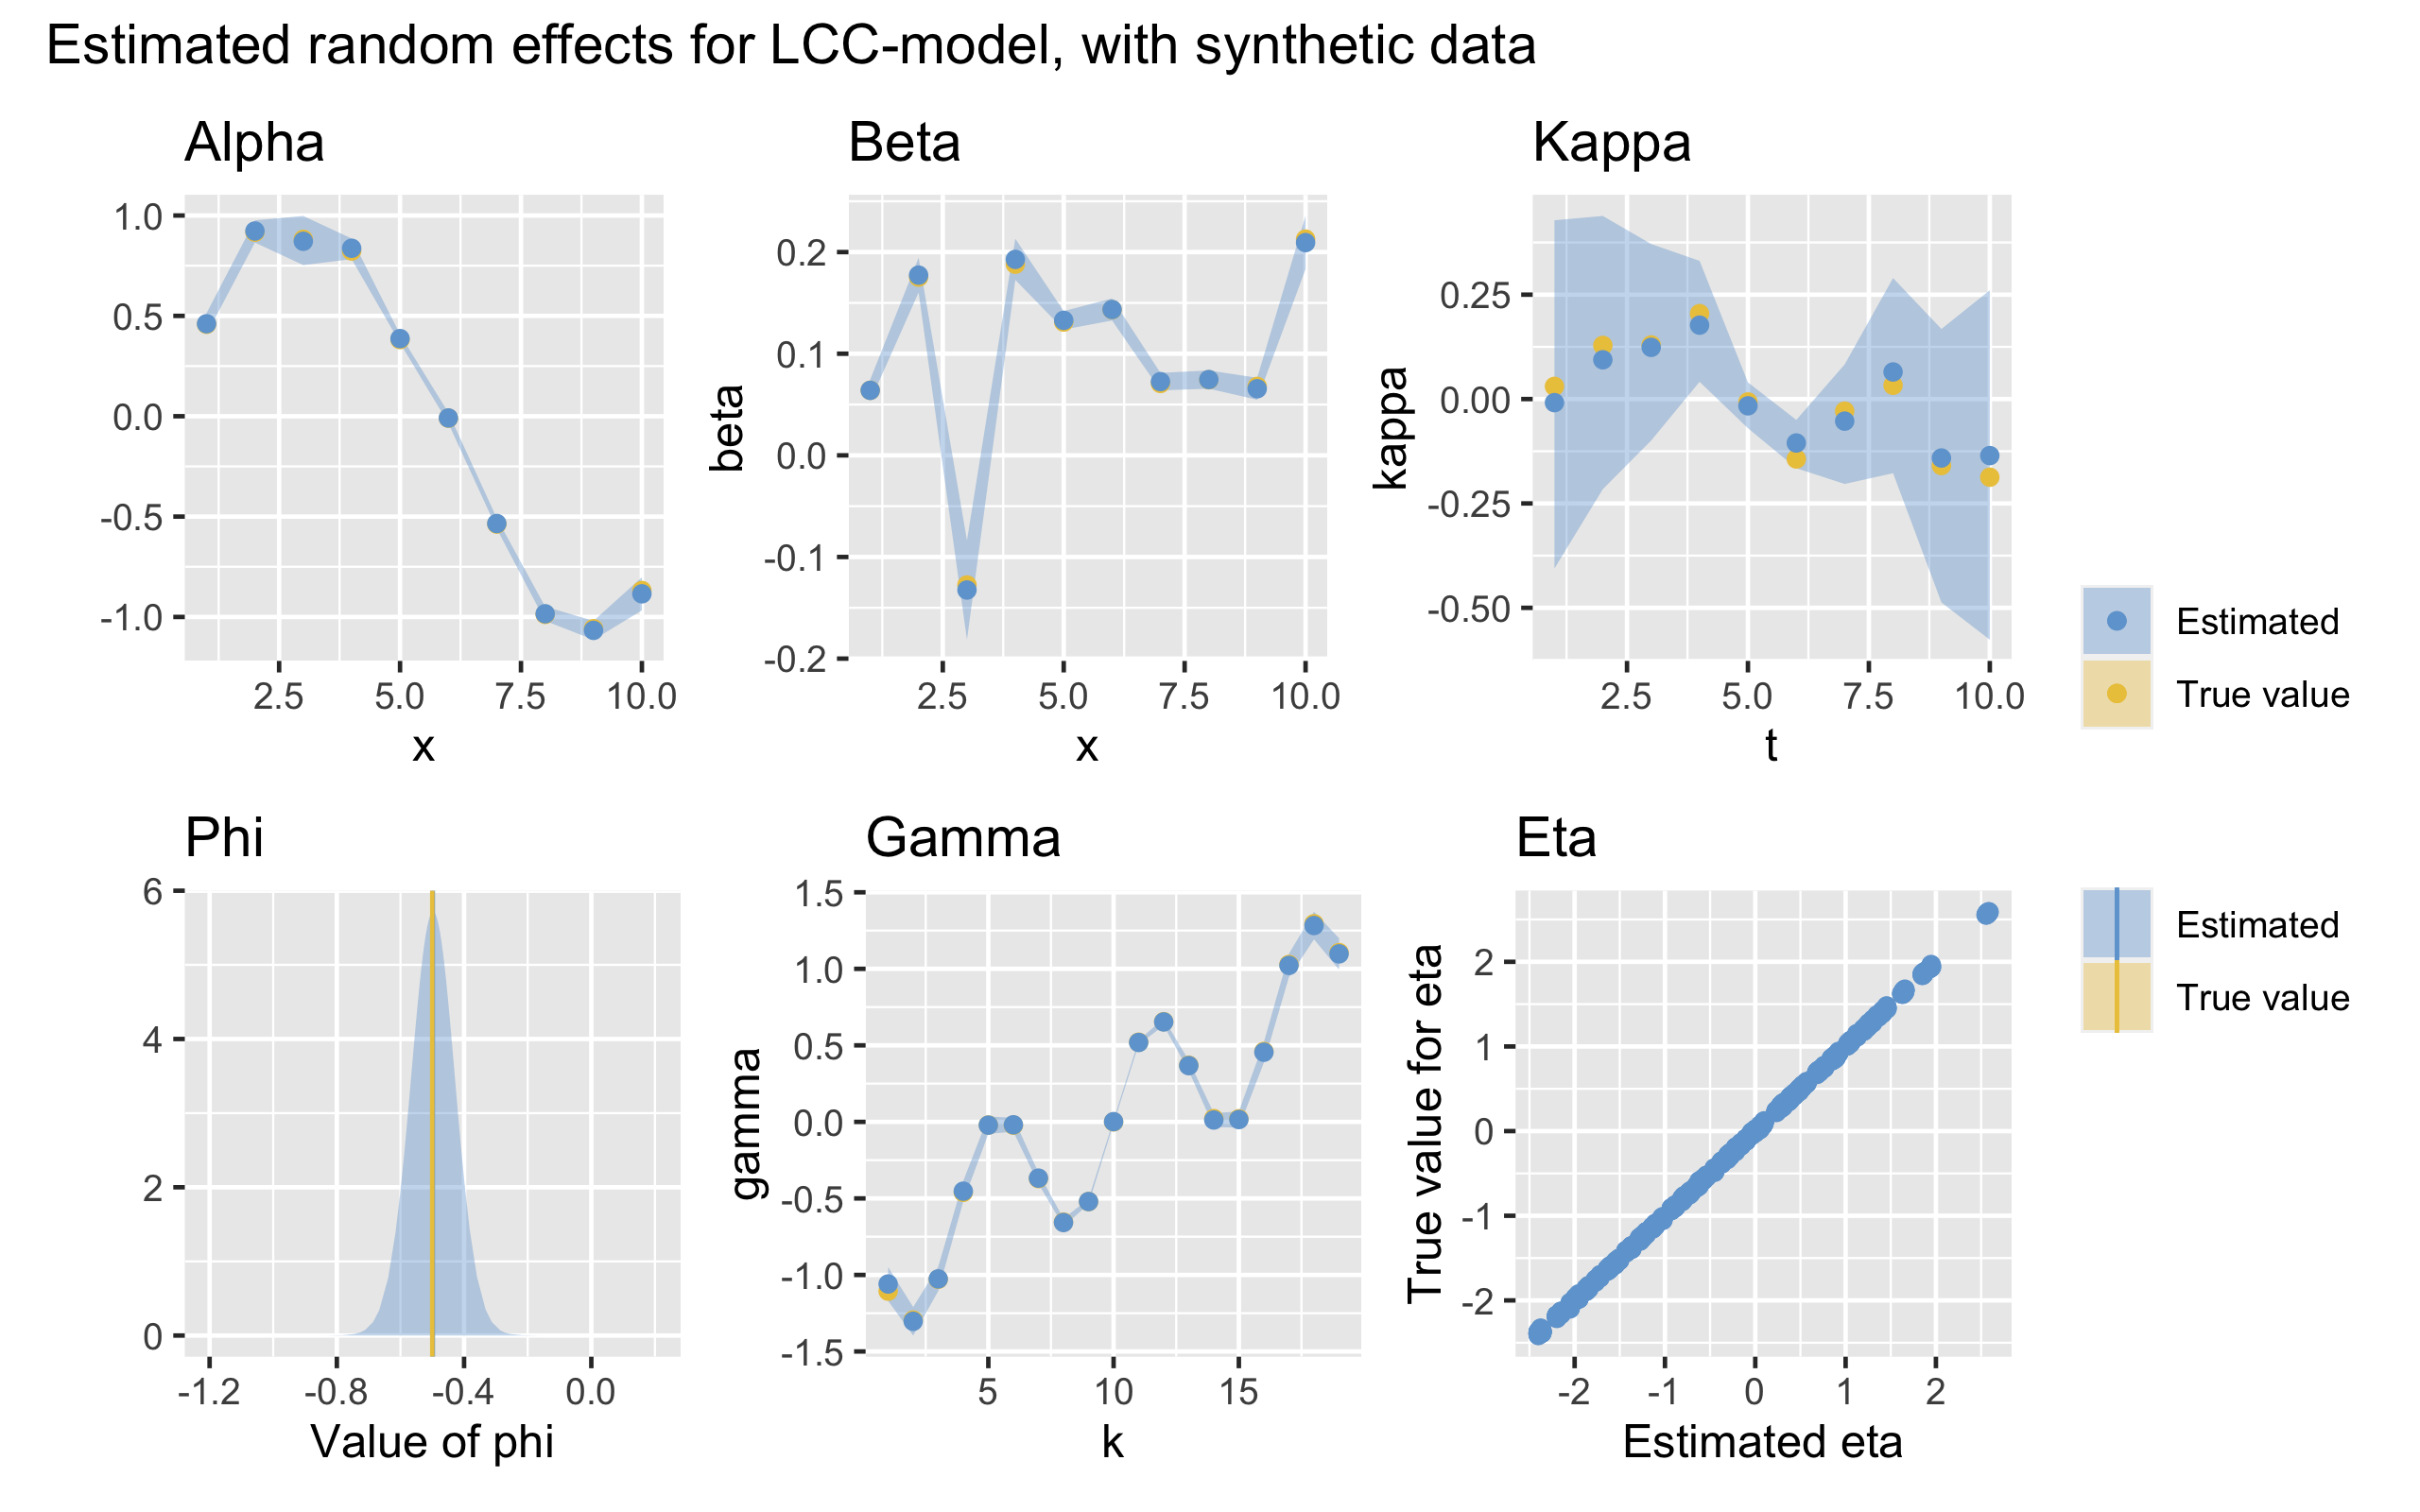
\includegraphics[width=0.85\linewidth]{synthetic-data/Figures/effects-LCC-synthetic-3-2.png}
    \caption{Results from running \inlabru with the configuration of random effects given in Expression \ref{eq:conf32}. The plot layout is similar to that of Figure \ref{fig:firstRun}.}
    \label{fig:conf32}
\end{figure}
Figure \ref{fig:conf32} displays the results from running \inlabru with the following configuration of random effects:
\begin{equation}
    \begin{aligned}
        &\alpha_x = \cos(\frac{x-3}{6}\pi) + \epsilon_{\alpha}, \quad \epsilon_{\alpha} \sim \Normal(0,0.05^2)\\
        &\beta_x = \Normal(0,0.1^2)\\
        &\phi = -0.5\\
        &\kappa_t = RW1(0,0.1^2)\\
        &\gammax = \frac{1}{2}\left( 0.2k + \sin(k)\right)\\
        &\tau_{\epsilon} = 1/0.01^2.
    \end{aligned}
    \label{eq:conf32}
\end{equation}
for $x\in[1,10]$, $t \in [1,10]$ and $k \in [1,19]$. 

\begin{figure}[h!]
    \centering
    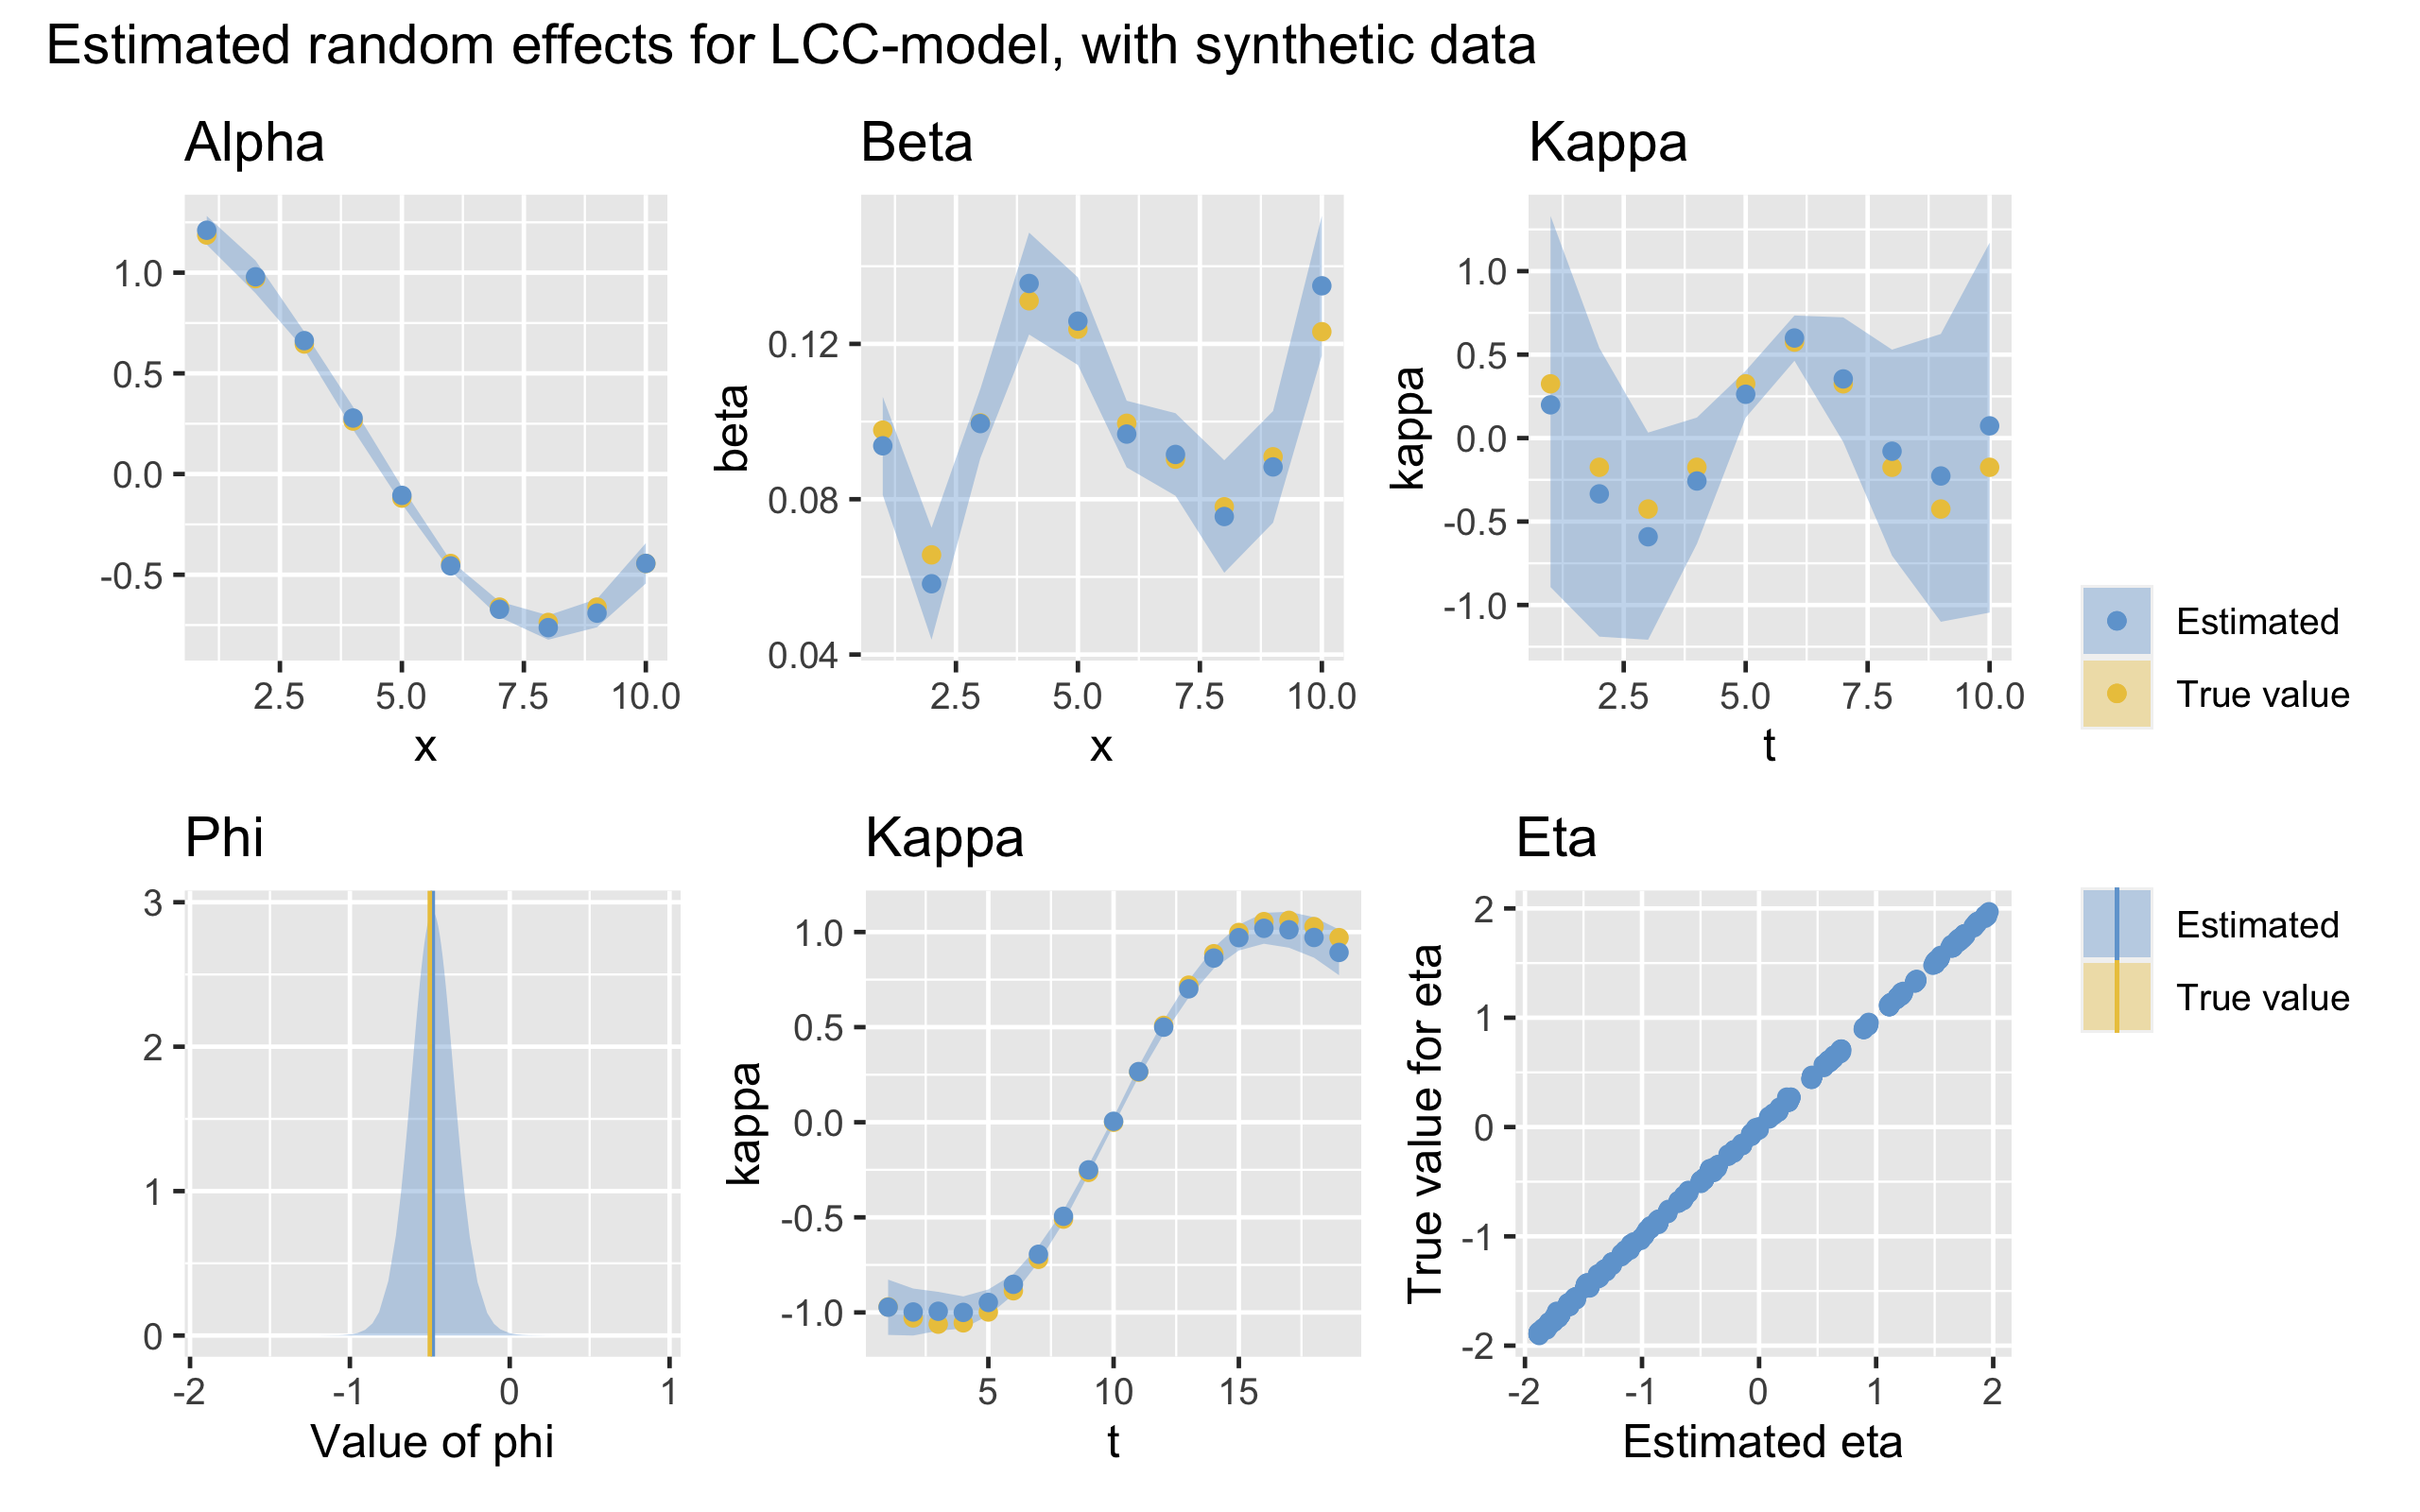
\includegraphics[width=0.85\linewidth]{synthetic-data/Figures/effects-LCC-synthetic-3-3.png}
    \caption{Results from running \inlabru with the configuration of random effects given in Expression \ref{eq:conf33}. The plot layout is similar to that of Figure \ref{fig:firstRun}.}
    \label{fig:conf33}
\end{figure}
Figure \ref{fig:conf33} displays the results from running \inlabru with the following configuration of random effects:
\begin{equation}
    \begin{aligned}
        &\alpha_x = \cos(\frac{x}{8}\pi)\\
        &\beta_x = \Normal(0,0.05^2)\\
        &\phi = -0.5\\
        &\kappa_t = \frac{1}{2}\cos(\frac{t\pi}{3})\\
        &\gammax = \frac{1}{2}\left( 0.2k + \sin(k/3)\right)\\
        &\tau_{\epsilon} = 1/0.01^2.
    \end{aligned}
    \label{eq:conf33}
\end{equation}
for $x\in[1,10]$, $t \in [1,10]$ and $k \in [1,19]$. 
From Figures \ref{fig:conf31}, \ref{fig:conf32} and \ref{fig:conf33} we observe that while the accuracy of the approximations is not as good as for the LC-model, \inlabru is still able to estimate the random effects for the LCC-model. The predictor $\eta_{x,t}$ is estimated well for all configurations. We do still observe some identifiability issues between $\kappa_t$, $\phi \cdot t$ (and to some degree $\alpha_x$ and $\beta_x$ as well), as can be seen in Figure \ref{fig:conf32}. However, when we test many different configurations, most results were not worse than the results displayed in Figure \ref{fig:conf32} (excluding the types of configurations discussed in Section \ref{sec:IdentifiabilityKappa}), and many results were accurate.  Considering this, we can still say that these results indicate that \inlabru is a suitable tool to perform Bayesian inference on LCC-models. 
